% !TEX root =  master.tex 
\chapter{UML-Diagramm -- Gemeinsam}

Da unser UML-Diagramm sehr groß ist, befindet sich hier ein Diagramm, das nur die vorhanden Klassen und deren Beziehungen beinhaltet:

\begin{minipage}{\linewidth}
	\centering
	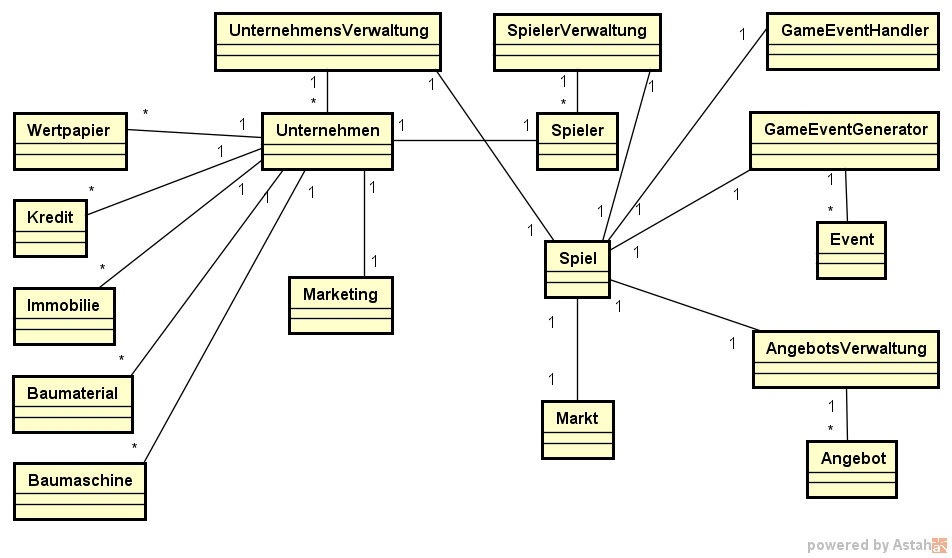
\includegraphics[scale=0.63]{img/ClassDiagramzweiteIterationFallstudieUEbersicht.png}
	\captionof{figure}{\label{abb:class1}UML-Diagramm (Klassenübersicht)}
	\vspace{2em}
\end{minipage}

Das vollständige UML-Diagramm befindet sich auf der nächsten Seite. Das Diagramm liegt zur besseren Lesbarkeit auch in digitaler Version vor.

\begin{minipage}{\linewidth}
	\centering
	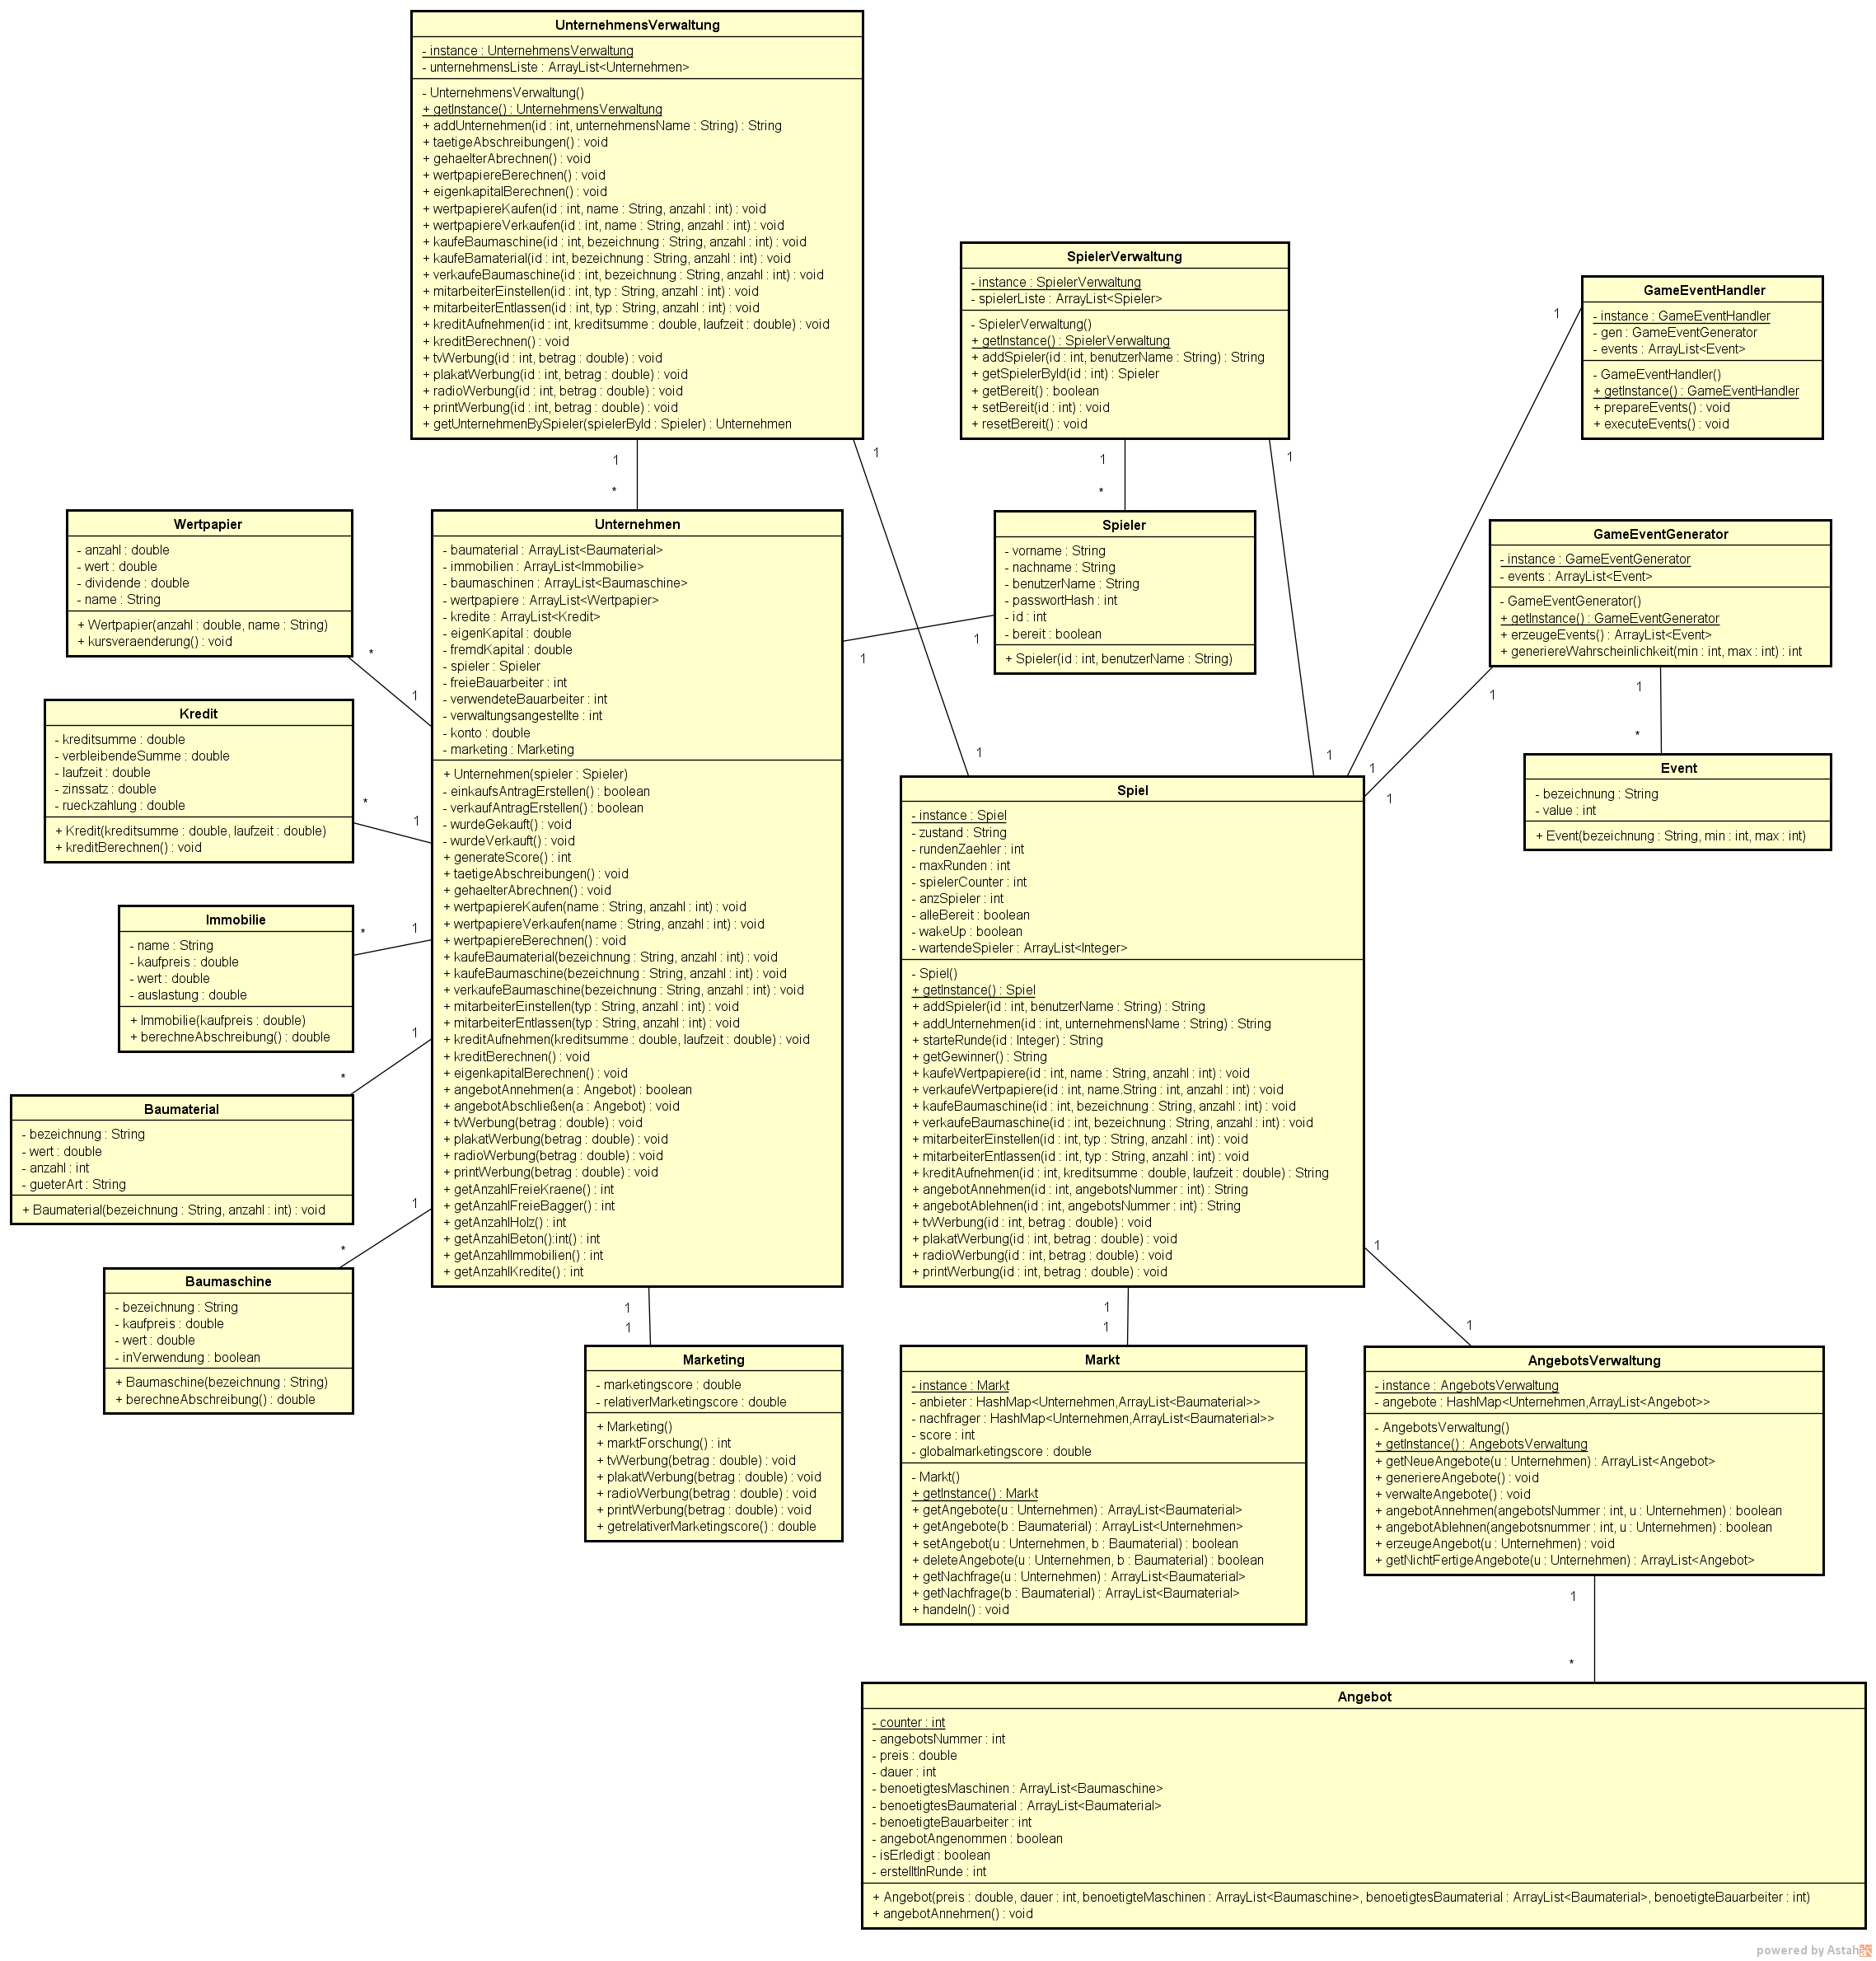
\includegraphics[scale=0.25]{img/ClassDiagramzweiteIterationFallstudie.png}
	\captionof{figure}{\label{abb:class2}UML-Diagramm}
	\vspace{2em}
\end{minipage}